%https://cloudconvert.com/pptx-to-eps
% convert power point to eps
In a cellular network, massive MIMO systems of $L$ cells, where a single BS per cell is equipped 
with $M$ antennas is considered. %and 
%serves simultaneously to $K_A$ active UEs. 
In this full spectrum reuse scenario, there are total $K$ UEs in the UE set $K_l\triangleq\{1,...,K\}$ in each cell $l$. Moreover, within this set, a number of $K_A$ active UEs in the subset $U_l$, $U_l\subset K_l$, are selected to be served in some resource blocks. Note that in this multi-cell network, the pilot sequence used by single-antenna UEs in the same
cell are assumed to be mutually orthogonal. Moreover, we assume the BSs are all synchronized in time. Furthermore, the pilot, UL and DL data are all aligned in the network.\footnote{There are alternative pilot structures. For example, to superimpose  the pilot sequences of one cell to the neighboring cells on their UL data transmissions\cite{upadhya2017superimposed}. Or some cells send UL pilots, while others send DL data \cite{fernandes2013inter}. As in this paper, rather than relying on adjusting the sequence length so as to decorrelate the channel estimation, we aim to collect the channel information wisely for pilot decontamination. Therefore, we choose to align all frame planning among multiple-cells.} The channel $\mathbf{h}_{jU_j[k]}\in\mathbb{C}^{M}$ from UE $U_j[k]$ to BS $j$ with a correlation due to finite multipath angular spread at the BS  can be represented as
\begin{equation}
\mathbf{h}_{jU_{j}[k]}=\beta_{jU_{j}[k]}\mathbf{R}_{jU_{j}[k]}^{1/2}\mathbf{h}_{W},
\end{equation}
where $\beta$ is the individual large scale fading gain, $\mathbf{R}_{jU_{j}[k]}$ is the second order channel covariance matrix and is defined as $\mathbf{R}_{jU_j[k]}=\E{({\mathbf{h}}_{jU_j[k]}{\mathbf{h}}_{jU_j[k]}^H)}$ and $\mathbf{h}_{W}\sim \mathcal{CN}\left(\mathbf{0},\mathbf{I}_M\right)$ stands for zero-mean complex Gaussian distribution with covariance $\mathbf{I}_M$. The covariance matrix R can be from measured channel or the local scattering spatial correlation model\cite{bjornson2017massive}, with the normalization $tr(\mathbf{R})=M$.

\subsection{CSI at the BS receiver}
A pilot sequence $\mathbf{\phi}_{U_j[k]}\in \mathbb{C}^{\tau} $ is transmitted by the $k_{th}$ UE in the UE set $U_j$ of cell $j$ for the UL channel estimation. $\tau$ denotes the length of pilot sequence in a coherence block, and sequence $\mathbf{{\phi}}$ which fulfills the constraint $\left\Vert\mathbf{\phi}\right\Vert^2=\tau$ is scaled by UE's transmit power $\sqrt{p}$ \footnote{Here we assume all UEs transmit the same power. }. As an orthogonal pilot codebook is assumed here, for two different pilot sequences, there is zero cross-correlation.  The received matrix in the $j_{th}$ BS is represented as 
\begin{equation} \label{eq:Yj}
\mathbf{Y}_j = \sqrt{p}\Big(\underbrace{\sum_{k = 1}^{K_A} \mathbf{h}_{jU_j[k]} \mathbf{\phi}_{U_j[k]}^T}_\text{Desired pilots} +\underbrace{\sum_{\substack{l=1 \\ l\neq j}}^{L}\sum_{k = 1}^{K_A} \mathbf{h}_{jU_l[k]} \mathbf{\phi}_{U_l[k]}^T}_\text{Inter-cell pilots}\Big) + \mathbf{N},   
\end{equation}
%where $\mathbf{h}_{jU_j[k]}\in\mathbb{C}^{M}$ stands for channel from UE $U_j[k]$ to BS $j$ and 
where $\mathbf{N}$ is the independent identically distributed
(i.i.d.) complex Gaussian noise with elements distributed as $\mathcal{CN\left(\mathit{0,N_o}\right)}$.
The BS then correlates the received pilot with $\mathbf{\phi}_{U_j[k]}^*$ to obtain the channel observation of $\mathbf{h}_{jU_j[k]}$:%.
\begin{equation} 
\mathbf{y}_{jU_j[k]} = \tau\sqrt{p}\Big(\underbrace{\mathbf{h}_{jU_j[k]}}_\text{Desired pilot} +\underbrace{\sum_{U_l[s]\in \\ \zeta\char`\\\{(l,s) = (j,k)\}}\mathbf{h}_{jU_l[s]}}_\text{Interfering pilots}\Big) + \tilde{\mathbf{n}}.   \label{eq:pilot contamination}
\end{equation}
Let $\zeta$ denotes a pilot reuse set which includes all UEs that share a common pilot sequence and can be defined as
\begin{equation}
%\begin{aligned}
\zeta \subseteq \{U_l[s]:\mathbf{\phi}_{U_j[k]}^T \mathbf{\phi}_{U_l[s]}^*=\tau, \{l=1,...,L;s=1,...,K_A\}\}.
%\end{aligned}
\end{equation}
Moreover, $\char`\\$ stands for excluding elements in the set. As shown in (\ref{eq:pilot contamination}), the interfering channel from the neighboring cells leak directly to the desired estimate.

\subsection{The Antenna Averaged Correlation Coefficient}
We temporarily assume that the second order channel covariance matrices are available. \cm{we will discuss this later}
In order to find the correlation metric for the desired and interfering channels as an input of deep learning model, we first look at only the channel estimation of the desired UE.
\begin{equation}
\hat{\mathbf{h}}^{Bay}_{jU_j[k]} = \sqrt{p}\mathbf{R}_{jU_j[k]} \mathbf{\Psi}_{jU_j[k]} \mathbf{y}_{jU_j[k]}, 
\end{equation}
where the superscript $Bay$ stands for the Bayesian channel estimation, $\sigma_{n}^{2}$ is the variance of regularized noise and $\mathbf{\Psi}_{jU_j[k]}$ is defined as

\begin{equation}
\mathbf{\Psi}_{jU_j[k]} = \Bigg(\tau\:{p}\sum_{U_l[s]\in\zeta} \mathbf{R}_{j,U_l[s]} + \sigma^2_n \mathbf{I}_M\Bigg)^{-1}.
\label{eq:psi_function}
\end{equation}

From \cite{bjornson2017massive}, we know if two UEs shared the same pilot sequence, the correlation of their channels can be defined as
\begin{equation}
\begin{split}
\rho={} &
\frac{\E\left\{ \left(\hat{\mathbf{h}}_{jU_{j}[k]}\right)^{H}\hat{\mathbf{h}}_{jU_{l}[s]}\right\} }{\sqrt{\E\left\{ \left\Vert \hat{\mathbf{h}}_{jU_{j}[k]}\right\Vert ^{2}\right\} \E\left\{ \left\Vert \hat{\mathbf{h}}_{jU_{l}[s]}\right\Vert ^{2}\right\} }}=\\
& \frac{tr\left(\mathbf{R}_{jU_{j}[k]}\mathbf{R}_{jU_{l}[s]}\mathbf{\Psi}_{jU_{j}[k]}\right)}{\sqrt{tr\left(\mathbf{R}_{jU_{j}[k]}\mathbf{R}_{jU_{j}[k]}\mathbf{\Psi}_{jU_{j}[k]}\right)tr\left(\mathbf{R}_{jU_{l}[s]}\mathbf{R}_{jU_{l}[s]}\mathbf{\Psi}_{jU_{j}[k]}\right)}}
\end{split}
\end{equation}

\subsection{Joint Bayesian Channel Estimation}
To facilitate the active UE set scheduling in order to avoid high inter-cell-interference, we modify the joint Bayesian channel estimator from \cite{yin2013coordinated}, which estimates channels from all cells simultaneously. By vectorizing the Bayesian channel estimate in the $\zeta$ set, we obtain $\hat{\mathbf{h}}_{\zeta}=[\hat{\mathbf{h}}_{jU_{1}[s_{1}]}^{T}...\hat{\mathbf{h}}_{jU_{L}[s_{L}]}^{T}]^{T},\:s_{l}\in \{\text{UEs in the set } \zeta\}$ 

\begin{equation}
\hat{\mathbf{h}}_{\zeta}^{Bay}=\mathbf{R}_{\zeta}\mathbf{S}^{T}(\mathbf{S}\mathbf{R}_{\zeta}\mathbf{S}^{T}+\sigma_{n}^{2}\mathbf{I}_{M})^{-1}\mathbf{y}_{jU_{j}[k]},
\end{equation}
where $\mathbf{R}_{\zeta}=diag\{\mathbf{R}_{jU_{1}[s_{1}],...,}\mathbf{R}_{jU_{L}[s_{L}]}\},\:s_{l}\in \{\text{UEs in the set } \zeta\}$ and $\mathbf{S}\triangleq[I_{M}...I_{M}]$ is a $M\times ML$ matrix.

% convert matlab to latex
%https://tex.stackexchange.com/questions/329308/how-to-convert-a-matlab-figure-to-a-latex-code-not-to-a-graphic

\begin{figure}[t!]
	\centering
	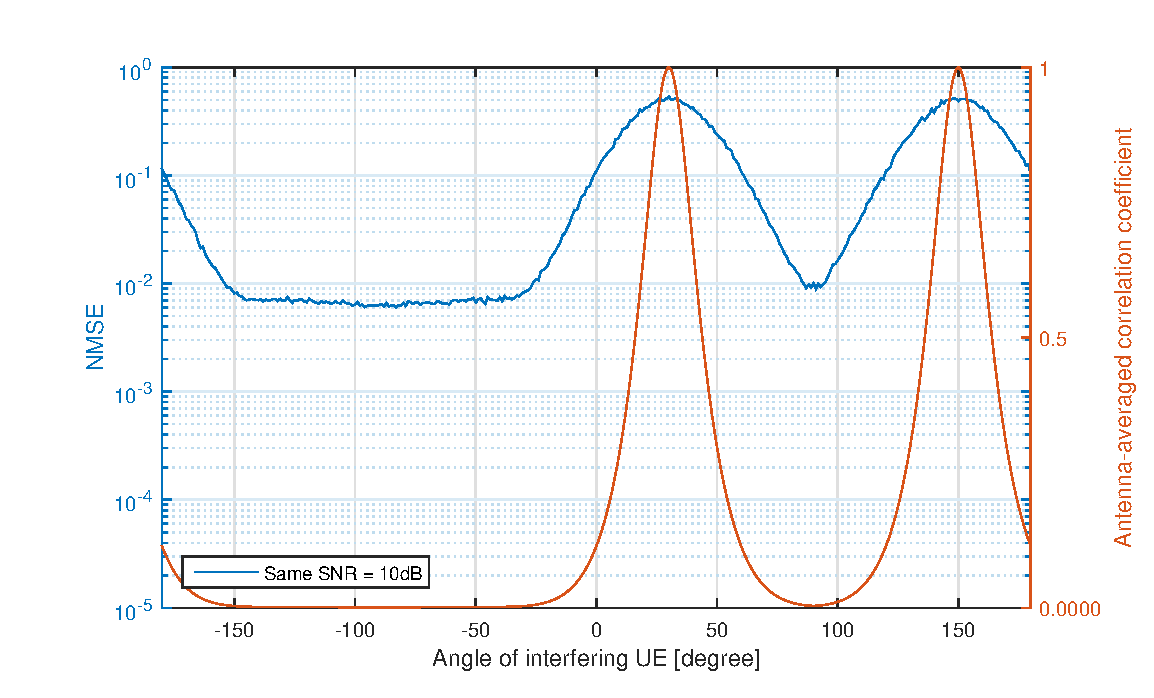
\includegraphics[width=1.0\linewidth]{figures/NMSE_correlation.eps}
	\caption{Correlation of NMSE channel estimation error to the antenna-averaged correlation coefficient. A spatially correlated channel, based on
the local scattering model with Gaussian angular distribution and ASD $ \sigma_\phi= 10^\circ$. The desired UE has a nominal angle of $30^\circ$, while the angle of the interfering UE
is varied between $−180^\circ$ and $180^\circ$}
	\label{fig:channel_correlation_model}
\end{figure}

\cm{introduce favorable condition for reducing inter-cell interference}


\begin{figure}[t!]
	\centering
	\includegraphics[width=1.0\linewidth]{figures/NMSE_correlation_measured_collocated.eps}
	\caption{Correlation of NMSE channel estimation error to the antenna-averaged correlation coefficient. A spatially correlated channel, based on
the measured correlation channel.}
	\label{fig:channel_correlation_measured}
\end{figure}


\cm{introduce favorable condition for reducing inter-cell interference}


\cm{introduction UL spectral efficiency which takes into account channel estimation errors}